\documentclass[12pt, a4paper]{article}
\usepackage{graphicx}
\usepackage{amsmath}
\usepackage{listings}

\title{Assignment 6(a) - Tubelight} % Title

\author{Jahnavi Pragada} % Author name

\date{\today} % Date for the report
\begin{document}
\maketitle
\section*{Introduction}
We use a 1-Dimensional model of the tubelight.  A uniform electric field is present, that accelerates electrons.  Electrons are emitted by the cathode with zero energy, and accelerate in this field.  When they get beyond a threshold energy, they can drive atoms to excited states. The relaxation of these atoms results in light emission.
\section*{TubeLight Model}
The tube is divided into n sections. In each time instant,M electrons are injected. We run the simulation for nk turns. The electrons are unable to excite the atoms till they have a velocity of u0. Beyond this velocity, there is a probability p in each turn that a collision will occur and an atom excited
\begin{verbatim}
    n=100 # spatial grid size.
    M=5 # number of electrons injected per turn.
    nk=500 # number of turns to simulate.
    u0=5 # threshold velocity.
    p=0.25 # probability that ionization will occur
\end{verbatim} 
We update xx and uu arrays taking acceleration to be $1$.The position and velocity of electrons which reached anode($xx>n$) are set to zero.
\begin{verbatim}
    ii=np.where(xx>0)[0] 
    dx[ii]=u[ii]+0.5         	
    xx[ii]=xx[ii]+dx[ii]     
    u[ii]=u[ii]+1            
    
    i_anode=np.where(xx>n)[0]
    xx[i_anode]=0
    u[i_anode]=0
    dx[i_anode]=0
\end{verbatim}
The electrons that have velocity more than threshold velocity and undergo collision are found . Now the positions of emitted electrons are added to intensity list I and their positions are updated.
\begin{verbatim}
    kk=np.where(u>=u0)[0]
    ll=np.where(np.random.rand(len(kk))<=p)[0]
    kl=kk[ll]
    u[kl]=0
    xx[kl]=xx[kl]-(dx[kl]*np.random.rand())
    I.extend(xx[kl].tolist())
\end{verbatim}
%This process is repeated for $nk$ turns.The graphs are plotted and the intensity data table is printed out in table format 
We find the positions in xx array which are unoccupied and inject the m new electrons in the unoccupied positions where m is given by the function $int(M+randn()*Msig)$\\ and initialize their position to 1
\begin{verbatim}
    Msig=2
    m=int((np.random.rand()*Msig)+M)
    iu=np.where(xx==0)[0]	
    xx[iu[:m]]=1
\end{verbatim}

\section*{Graphs}
Graphs are plotted using hist() and intensity table is printed out. Graphs of electron density,light intensity,electron phase space are plotted in figure 1,2,3.

\begin{figure}[!tbh]
\centering
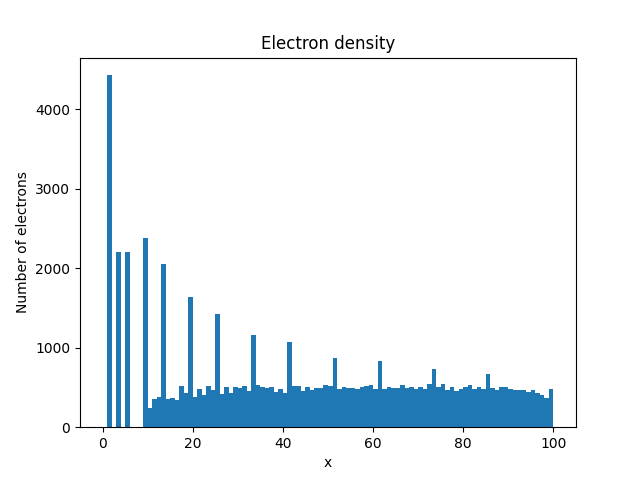
\includegraphics[scale=0.70]{Plot2.png}
\caption{Electron Density Graph}
\label{Figure1}
\end{figure}

\begin{figure}[!tbh]
\centering
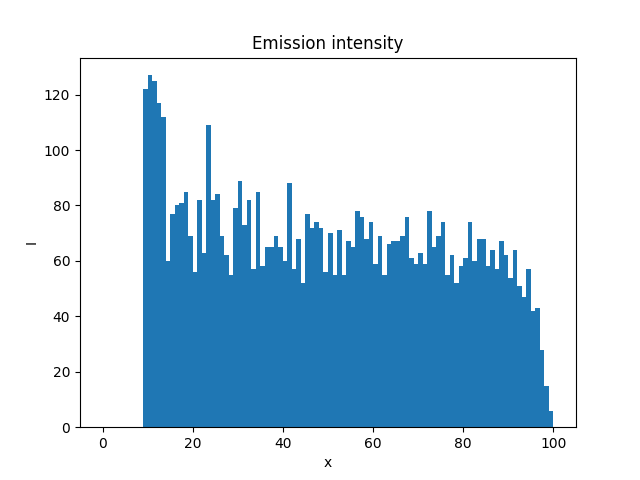
\includegraphics[scale=0.70]{Plot3.png}
\caption{Emission Intensity Graph}
\label{Figure2}
\end{figure}

\begin{figure}[!tbh]
\centering
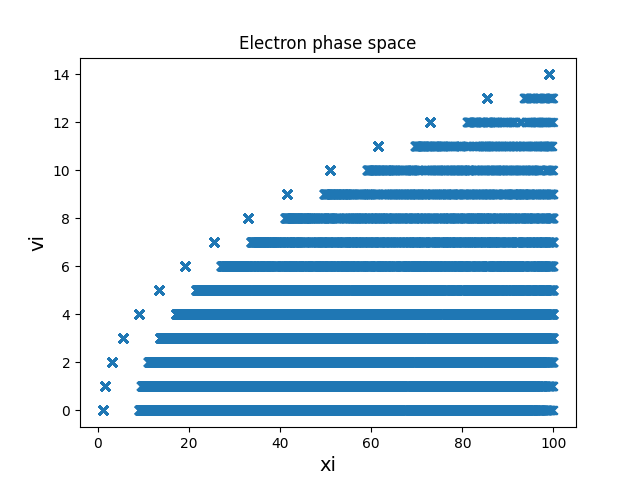
\includegraphics[scale=0.70]{Plot1.png}
\caption{Electron phase space Graph}
\label{Figure3}
\end{figure}


\section*{Conclusion}
We stimulated a tubelight model and plotted the graphs of Intensity,Electron position and electron phase space. We find that until 20,there is no much intensity.This is because the electrons there have velocity less than threshold velocity and are building up energy there.After that the emission decays because fewer energetic electrons reach there before colliding. At 40 we get next peak which is a diffuse since the zero energy location of different electrons is different.


\end{document}